\section{Task 3.3}
In order to project the Mamdani Fuzzy Inference System of this task, an analysis of the three best features of \verb|sequentialfs| has been done. In particular, were studied the \textbf{empirical distributions} of the features through some histograms. Then, a \textbf{correlation study} has been carried out by plotting scatter-plots with different combinations of pairs of these three features. In the following are presented those results:

\begin{figure}[H]
	\centering
	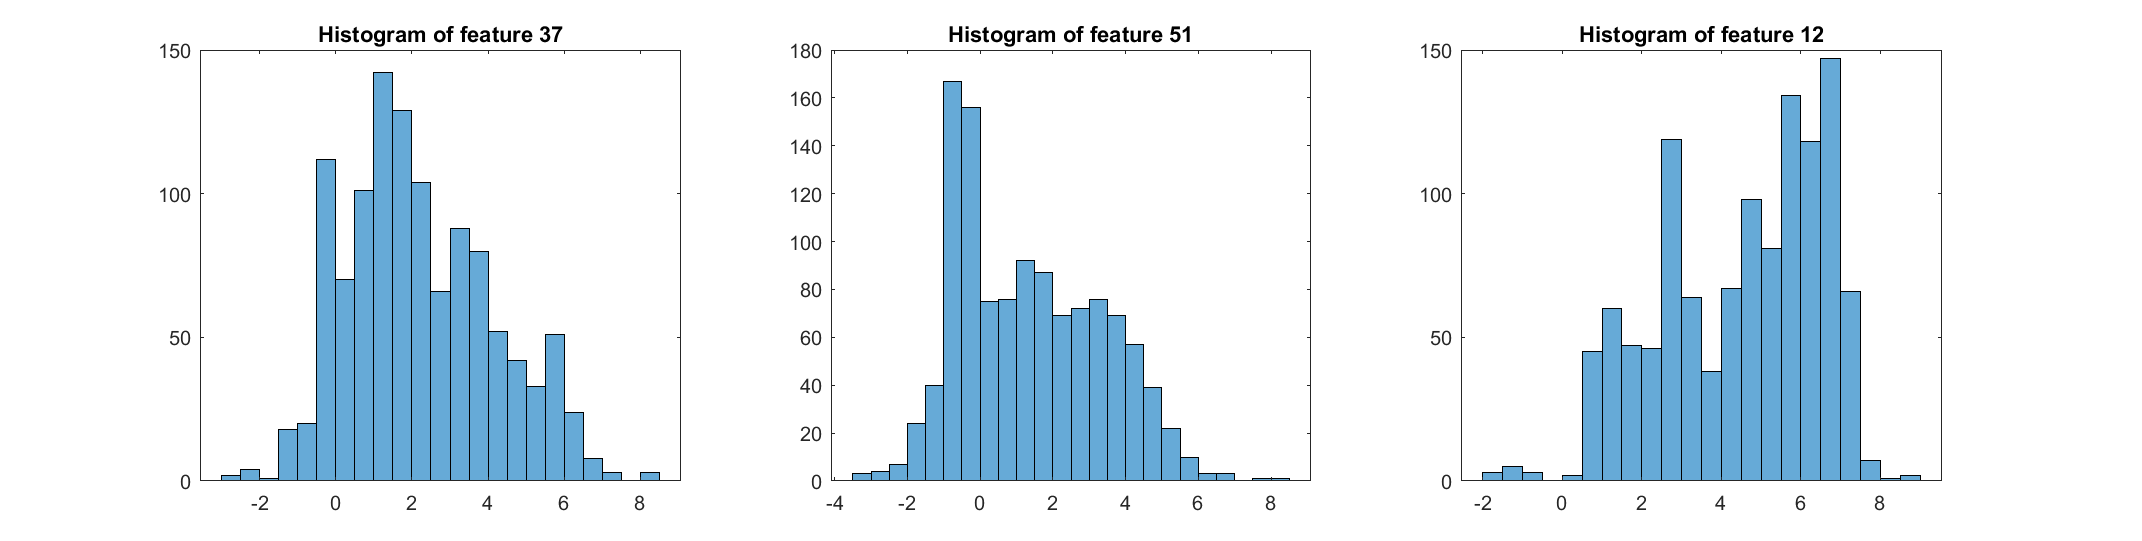
\includegraphics[width=\linewidth]{img/histogram_top_3_features.png}
	\caption{Histograms of three features}
\end{figure}

The empirical distribution has been used to model the linguistic variables of the three features. The approach adopted was the following: since the empirical distributions are "fuzzy", but also tends to have peaks in some points, those peaks were considered as central point of a particular linguistic label.

\begin{figure}[H]
	\centering
	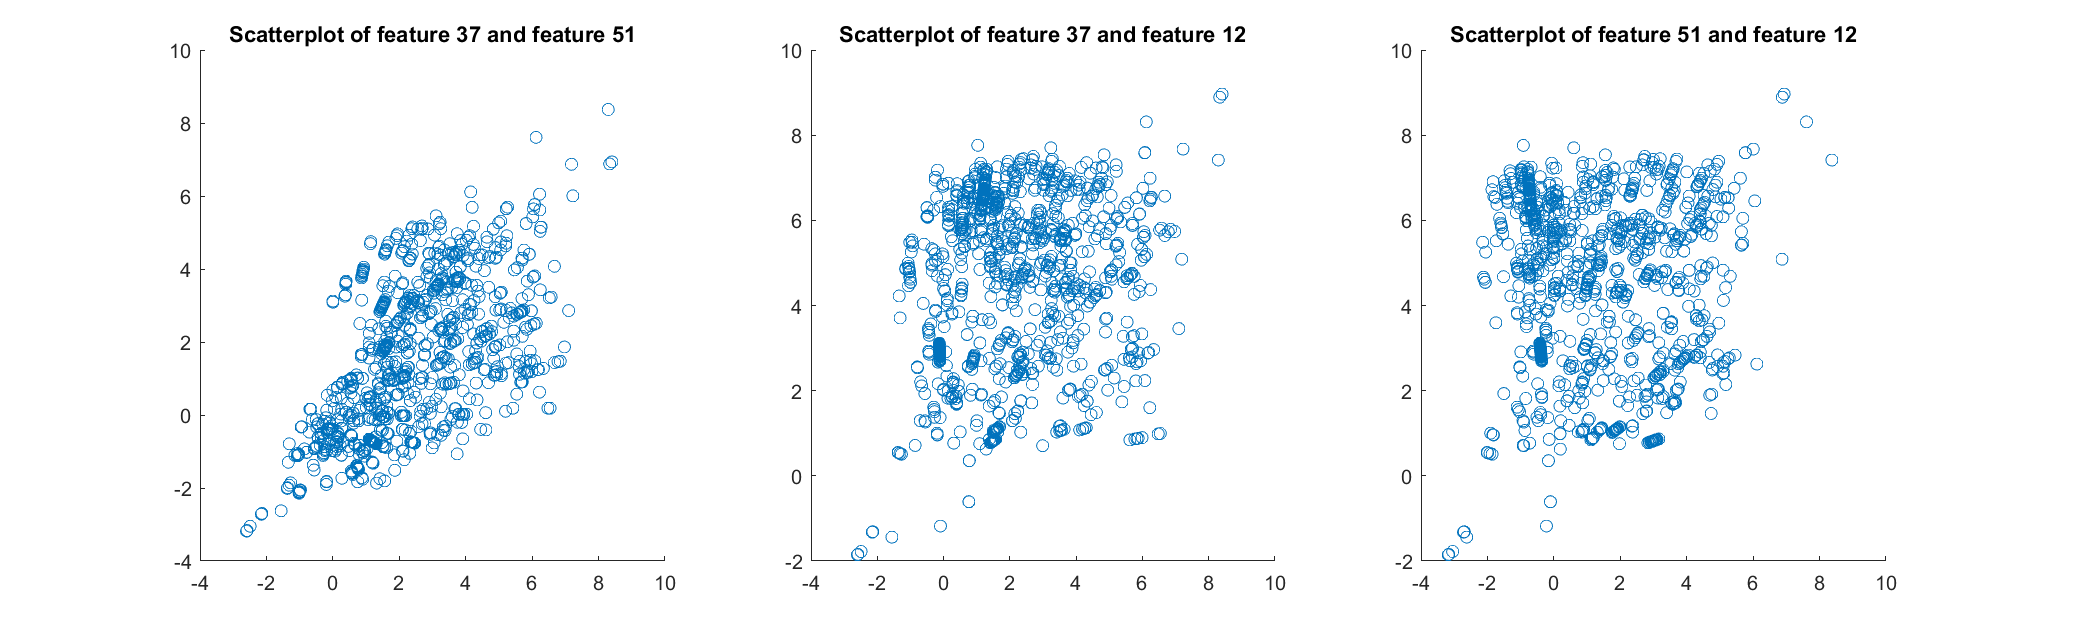
\includegraphics[width=\linewidth]{img/scatter_top_3_features.png}
	\caption{Scatter-plot of pairs of features}
\end{figure}

By watching the scatter-plot, we can see a certain positive correlation between feature 37 and 51 in the scatter-plot on the left, while other pairs seems uncorrelated due to the fact that the plot looks "square" without a particular tendency like the first one. \\
As a conclusion,in the antecedent of a fuzzy rule, an high(low) level of feature 37 with low(high) level of feature 51 won't be used due to their positive correlation.\\

So, for what concerns modeling of the linguistic variables of the \textbf{inputs}, when three linguistic labels were applied the central membership function was selected as a \textbf{triangle} while on the sides a \textbf{trapezoidal} membership function to cover all the universe of discourse of that particular feature.\\ As stated before the position of the various membership function was done w.r.t. the peaks of the empirical distribution of features. \\

They inputs has been modeled as follows:
\begin{figure}[H]
	\centering
	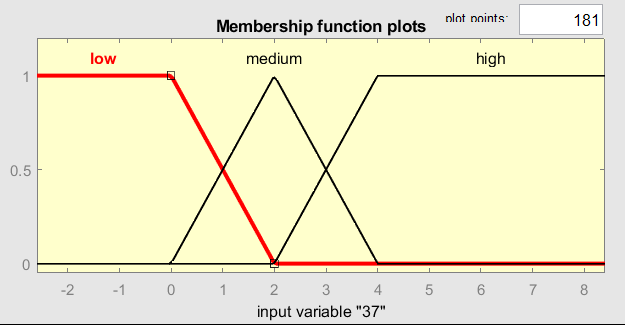
\includegraphics[width=0.5\linewidth]{img/lin_var_37.png}
	\caption{Modeling of linguistic variable of the input for feature 37}
\end{figure}
\begin{figure}[H]
	\centering
	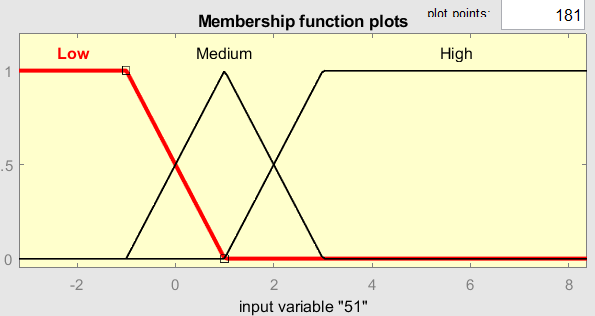
\includegraphics[width=0.5\linewidth]{img/lin_var_51.png}
	\caption{Modeling of linguistic variable of the input for feature 51}
\end{figure}
\begin{figure}[H]
	\centering
	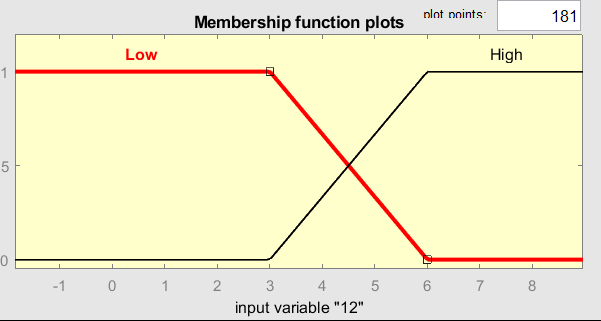
\includegraphics[width=0.5\linewidth]{img/lin_var_12.png}
	\caption{Modeling of linguistic variable of the input for feature 12}
\end{figure}

For the arousal linguistic variable \textbf{output}, since the input data is not particularly "defined" but has some uncertainty in the histograms, the output has been modeled in only three different linguistic labels with triangular membership function otherwise creating some fuzzy rules was very complicate:
 \begin{figure}[H]
 	\centering
 	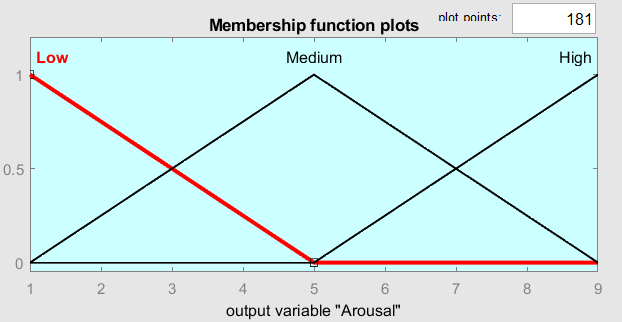
\includegraphics[width=0.5\linewidth]{img/lin_var_arousal.png}
 	\caption{Modeling of linguistic variable of the arousal output}
 \end{figure}
For what concerns the rules, other histograms were plotted, this time by only considering a subset of the samples coinciding to a specific range of arousal. Some samples were not considering in the modeling of the rules (red dotted line is used as a threshold).

\begin{figure}[H]
	\centering
	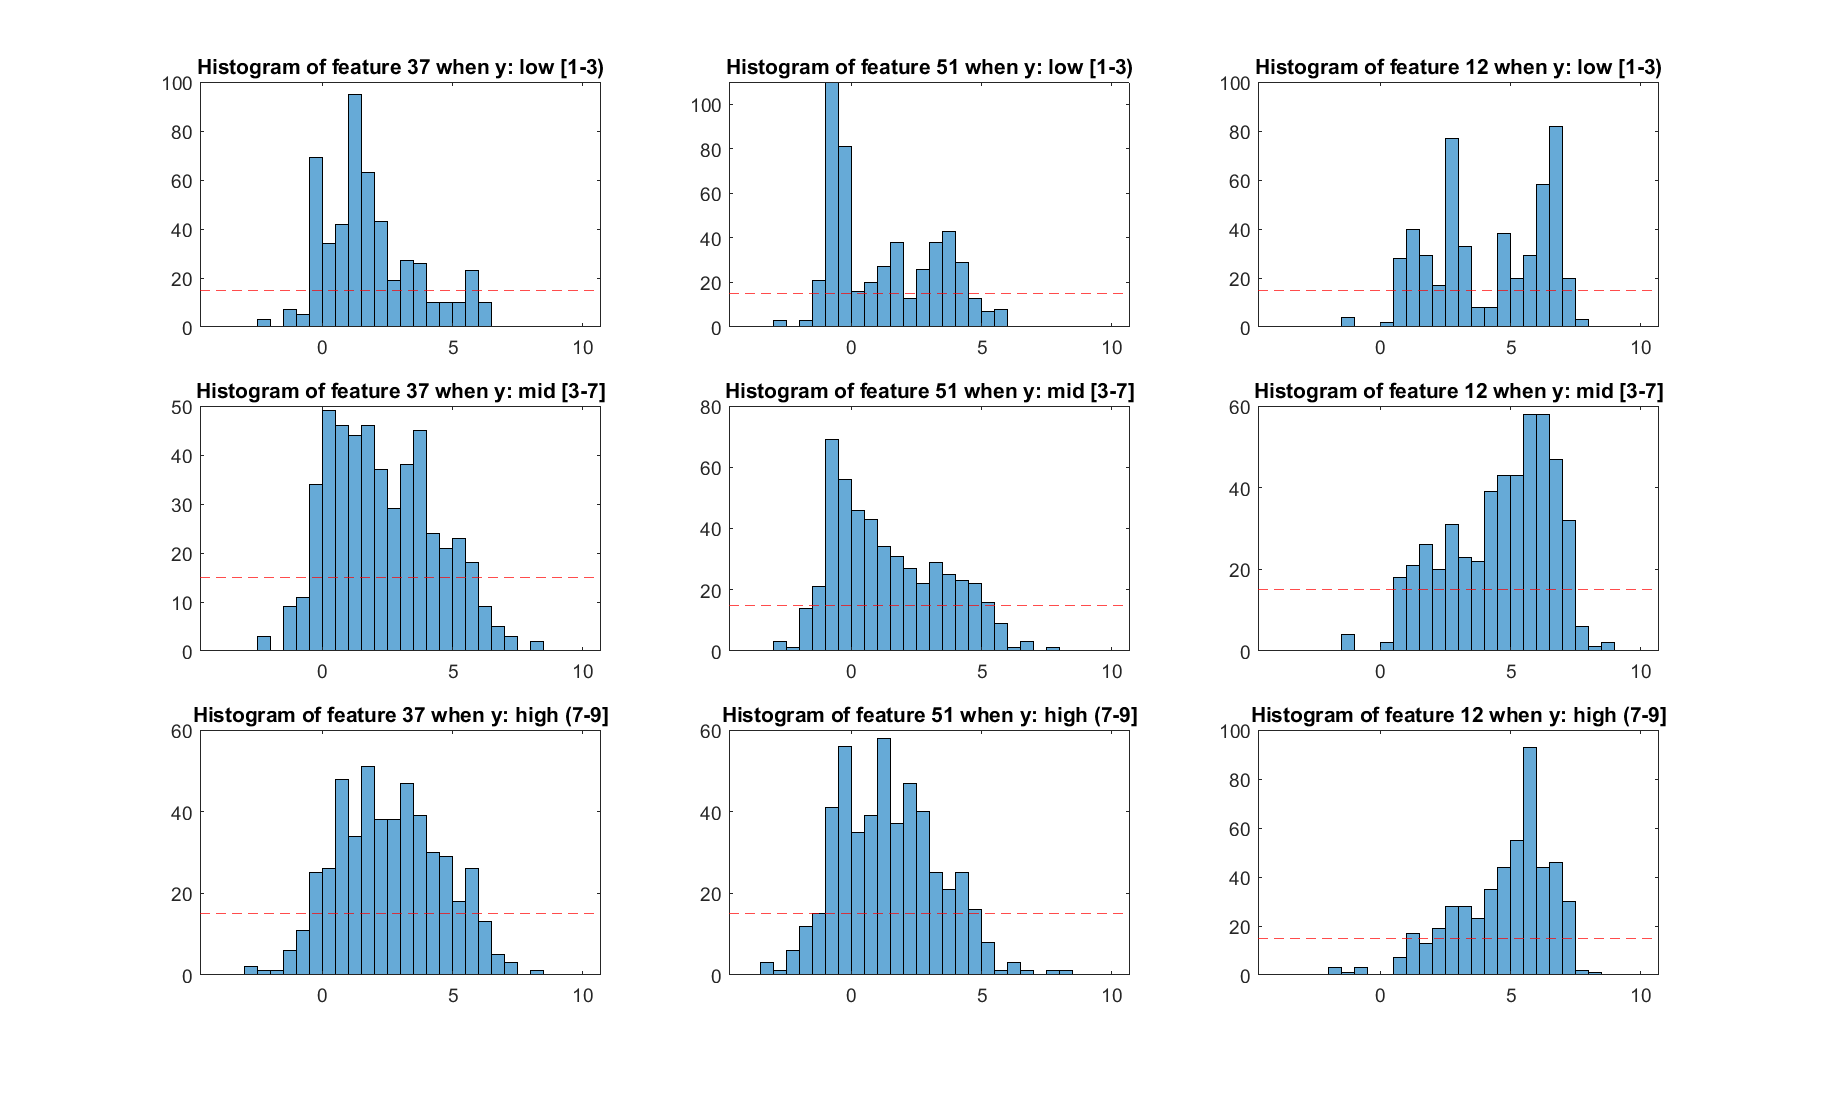
\includegraphics[width=\linewidth]{img/histogram_top_3_features_specific.png}
	\caption{Histograms of three features with ranges of arousal}
\end{figure}
The rules modeled are the following:
\begin{figure}[H]
	\centering
	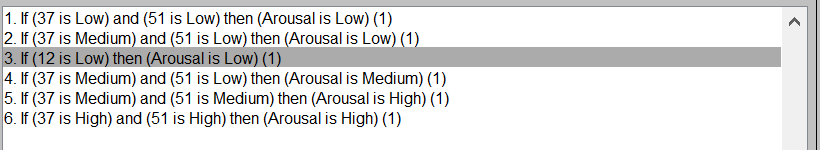
\includegraphics[width=\linewidth]{img/rules.png}
	\caption{Fuzzy Rules}
\end{figure}
For example: rule 3 was defined since only in the first histogram of feature 12 "lower" values appear. For features 37 and 31 was not very simple to find patterns so, at the end, the rules were generated by respecting the statement on the correlation above and comparing the positions of the peaks.  

